\chapter{Prototype \#2}

This chapter describes the chronology of this project's second prototype...

\section{Conception}

* This prototype's purpose was to explore possible input mechanisms.\\
** The past work outlined in Chapter 2 provided some guidance on how to begin:\\
- Researchers indicated the importance that inputs be based on already-present activities in the given environment (Barkhuus \& Jorgensen, 2008). Furthermore, others noted increased satisfaction from full-body movement as input (Ulyate \& Biancardi, 2001), and this goes well with the apparent subconscious ties between music and movement (Jourdain, 1997; Levitin, 2006). Thus, I created multiple input mechanisms based on some crowd behaviours -- clapping, swaying arms, doing `the wave,' holding up lighters, giving a thumbs up or thumbs down, and dancing.\\
- Researchers stressed the importance of immediate, obvious, and meaningful feedback (Ulyate \& Biancardi, 2001). I incorporated straightforward visual feedback for each input mechanism.\\
** I was given the opportunity to install work at an exhibition -- eLeo, an interactive show held at OCAD University. I modified my program to run on a loop such that users could engage with it without my facilitation.
% Background:
% Auslander, 1999: Communities are formed based on how the audience interacts, with no dependence on the spectacle at hand
% Turino, 2008:
% * Artists can shift between participatory and presentational performance
% * Different roles of different difficult allow for everyone to feel welcome and achieve flow. "Core" and "elaboration" roles cater to advanced and non-advanced performers respectively.
% * Open form: Basic motives repeated over and over. Easy for newcomers to join in. "Security in constancy." Can facilitate flow.
% * Hall: Repetition can increase intensity. Synchronicity comforts people.
% * Wide tuning, loud volumes, and overlapping textures provide a ``cloaking function'' that makes people more comfortable participating
% * Virtuosic solos are not common
% * Some participatory performances are sequential -- everyone gets a turn (e.g. Karaoke)
% Kelly, 2007: Displaying clips and themes from her music videos at a Madonna concert creates feelings of a "shared past" in the audience. (How might we create instead a "shared present"?)
% Small, 1998: Performers dressing in uniform are separating themselves and their responsibilities
% Davidson, 1997:
% * Performance etiquette is usually formed by crowd mentality, following the majority
% * Performers pick up information from the audience's broad and specific behaviours
% * Visuals help audiences read the performer's intentions
% Sexton, 2007: Simple synchronous interactions in sound art projects left users with little to explore, resulting in a "flat" experience
% Jourdain, 1997: We move to music in order to "represent" it. This also amplifies, resonates the musical experience.
% Levitin, 2006:
% * "In every society of which we're aware, music and dance are inseparable." Ancient music was based on rhythm and movement. Combining rhythm and melody bridges our cerebellum and cerebral cortex.
% * Ties between music and movement have only been minimized in the last 100 years
% Kelly, 2007: Technology incorporated into a show can either be addressed as part of the show or hidden and made illusory
% Maynes-Aminzade, 2002:
% * Computer vision: Movement-based control were intuitive, but camera required frequent calibration
% * Beach ball: Using a single beach ball as an input was also intuitive, but it only involved a few people at a time
% * Laser pointers: Gave everyone an individual cursor, but got chaotic once more and more people joined
% * Recommendations: Focus on compelling activity over impressive technology. Not everyone must be sensed as long as they feel involved. The control mechanism should be obvious or the users will give up. Make the activity emotionally engaging. Emphasize cooperation.
% Ulyate, 2001:
% * Design guidelines:
% * * Encourage and reward movement
% * * Feedback should be immediate, obvious, and meaningful in the context of the space
% * * No instruction or thinking should be required
% * * Responsiveness is more important than aesthetics
% * *  Modularity is key
% * Lessons learned:
% * * Full-body movement is most satisfying
% * * Form of the object determines how users interact
% * * A practical system is distributed and scalable
% * * Find balance between freedom and constraint
% * * Users will always find a way to create unwanted outputs
% * * Simple, instant gratification is important for feedback
% Barkhuus, 2008:
% * Inputs based on already-present behaviour lead to intuitive systems
% * Don't focus on employing cutting edge technology
% * Events should not rely on the success of the technology
% * Immediate visual or aural feedback is key
% Tseng, 2012: Being excluded from the interaction did not lessen enjoyment of the show
% Reeves, 2010:
% * "Intra-crowd interaction" is a common phenomena to exploit
% * Many actions "snowball" and overtake crowds; highly visible/audible actions promote this
% * People on the fringes of the crowd interact, but there is latency
% * Every crowd is different; designs should reflect the environment
% Gates, 2006: Technologies should reflect the performer's art and not be a burden on them


\section{Prototyping}

I first created a Max patcher that reads various movement data from the controller and visualizes them as different motions that a typical concertgoer might perform. The motions are: giving a ``thumbs up" or ``thumbs down", swaying arms from side to side, clapping, or doing ``the wave," as shown in Figure \ref{prototyping2.1}. Visual feedback is provided in the form of illuminated LED objects and moving sliders.

\begin{figure}[t]
	\centering

	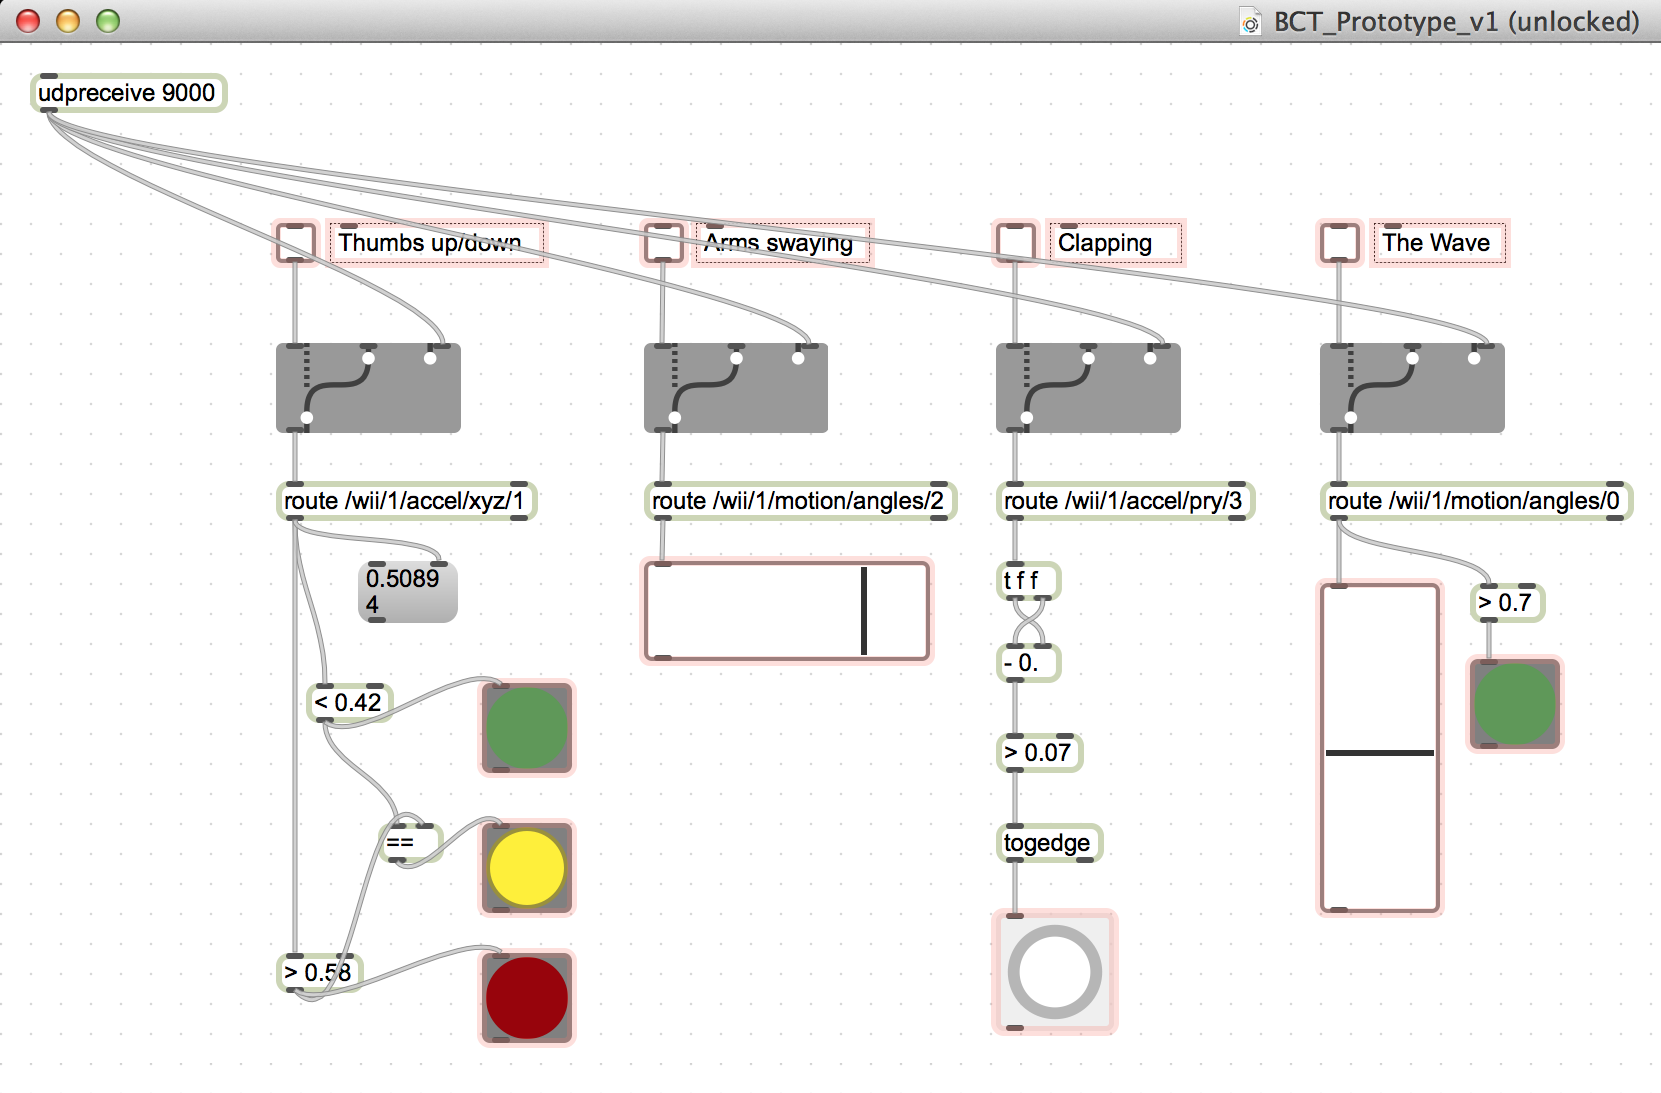
\includegraphics[height=0.3\textwidth]{wiimote_audience.png}
	\caption{Audience inputs}

	\label{prototyping2.1}
\end{figure}

\begin{figure}[t]
	\centering

	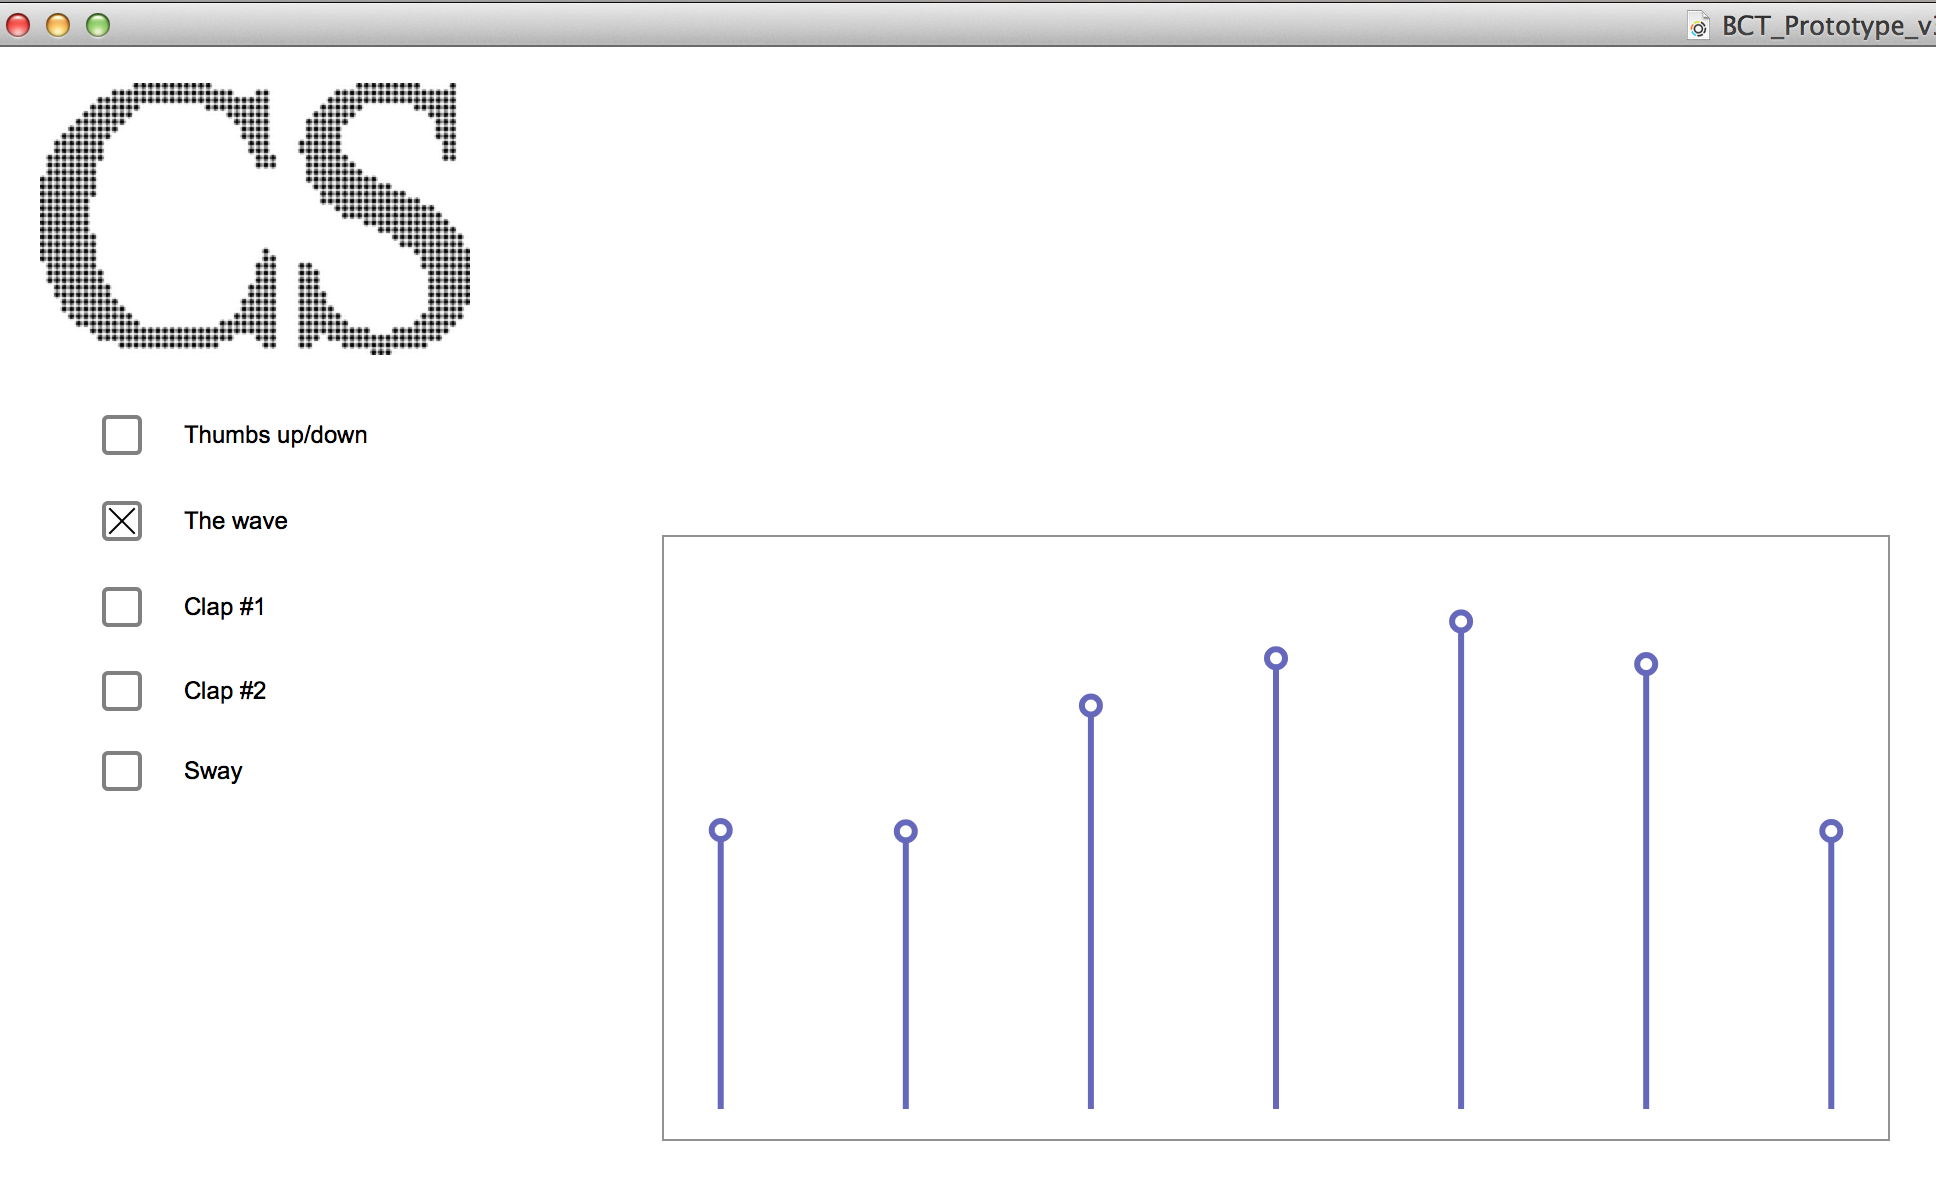
\includegraphics[height=0.3\textwidth]{the_wave.png}
	\caption{Audience inputs with seven users}

	\label{prototyping2.2}
\end{figure}

* I programmed the patcher to allow for seven users and created a presentation mode that provided visual feedback for everyone's actions. Figure \ref{prototyping2.2} shows the display for `the wave' mode. The clapping input was divided into two modes -- a `clap-o-meter' that displays applause intensity and a mode that encourages users to clap in sync.\\
** I update the visuals and added an auto-play function (Figure \ref{prototyping2.3}). This automatically flips through every round, playing each for a set amount of time.\\
** I added Lighters and Dance modes.\\
** I integrated video crossfade voting system within each mode, similar to Prototype \# 1.\\
** The prototype was installed at the eLeo exhibit (Figure \ref{prototyping2.4}).\\
%** Added sub-patcher to lighten the processing load.\\
%** Polished off presentation mode.\\

\begin{figure}[t]
	\centering

	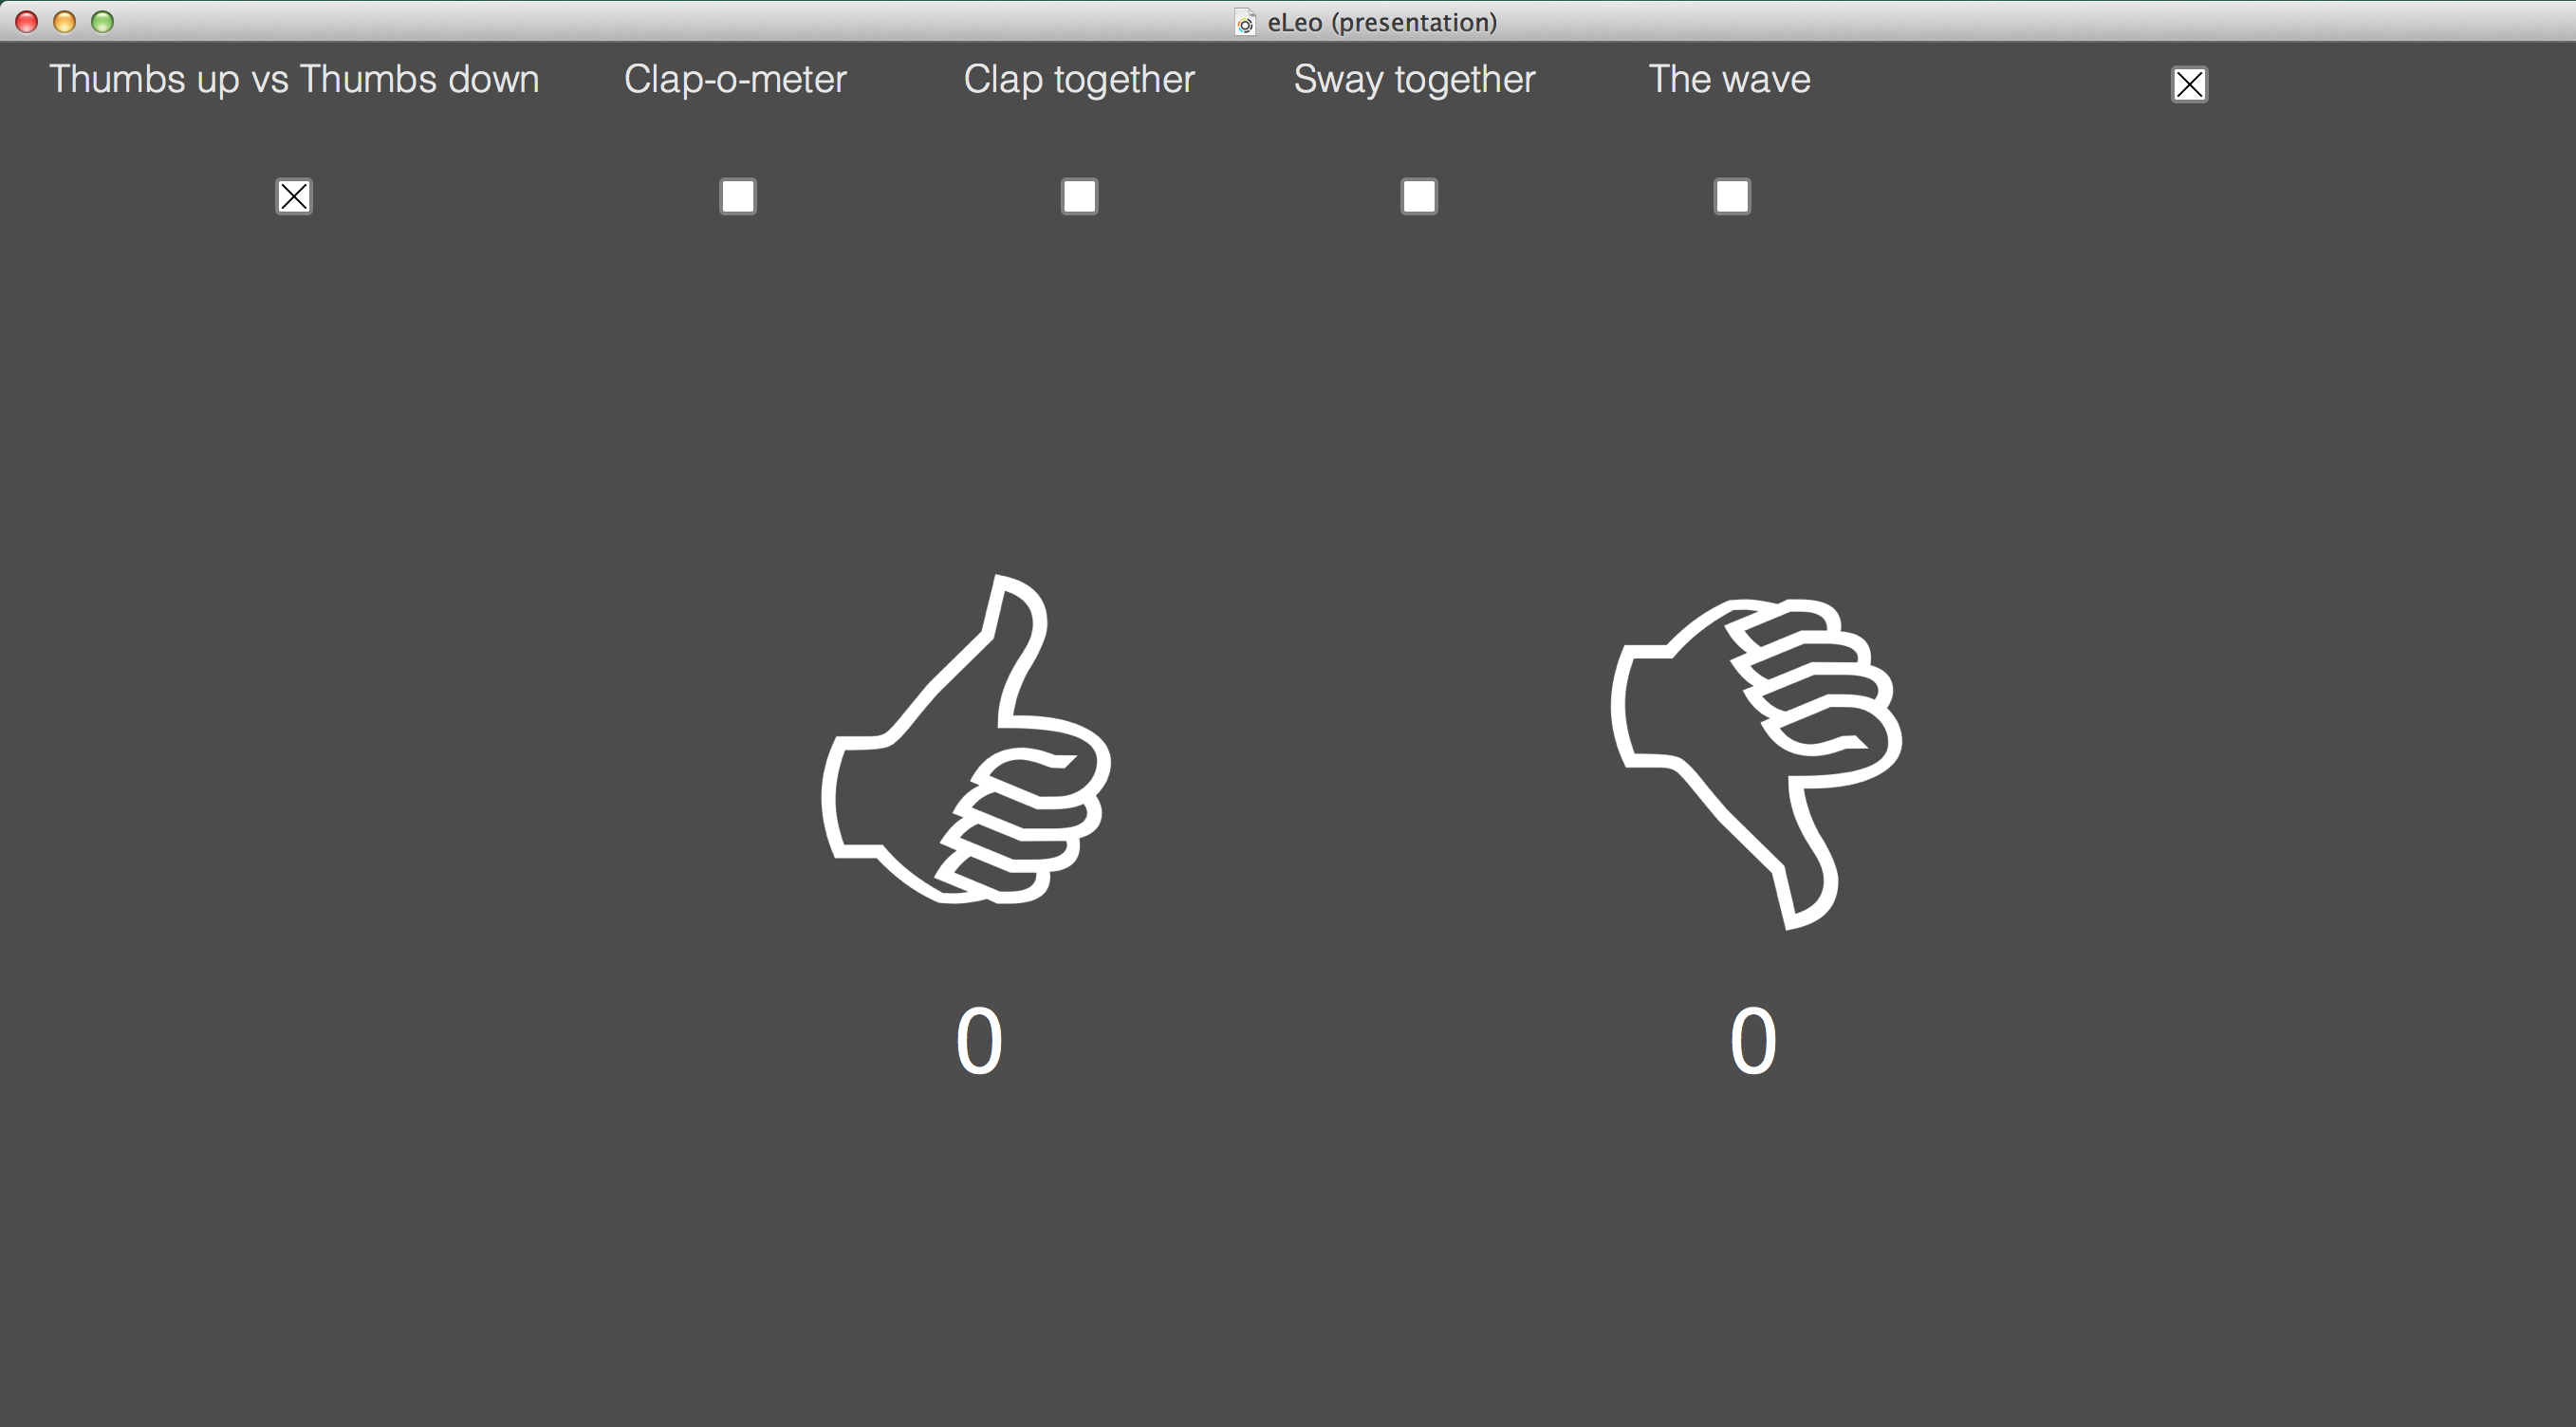
\includegraphics[height=0.3\textwidth]{eleo.png}
	\caption{Auto-play version for eLeo exhibit}

	\label{prototyping2.3}
\end{figure}

\begin{figure}[t]
	\centering

	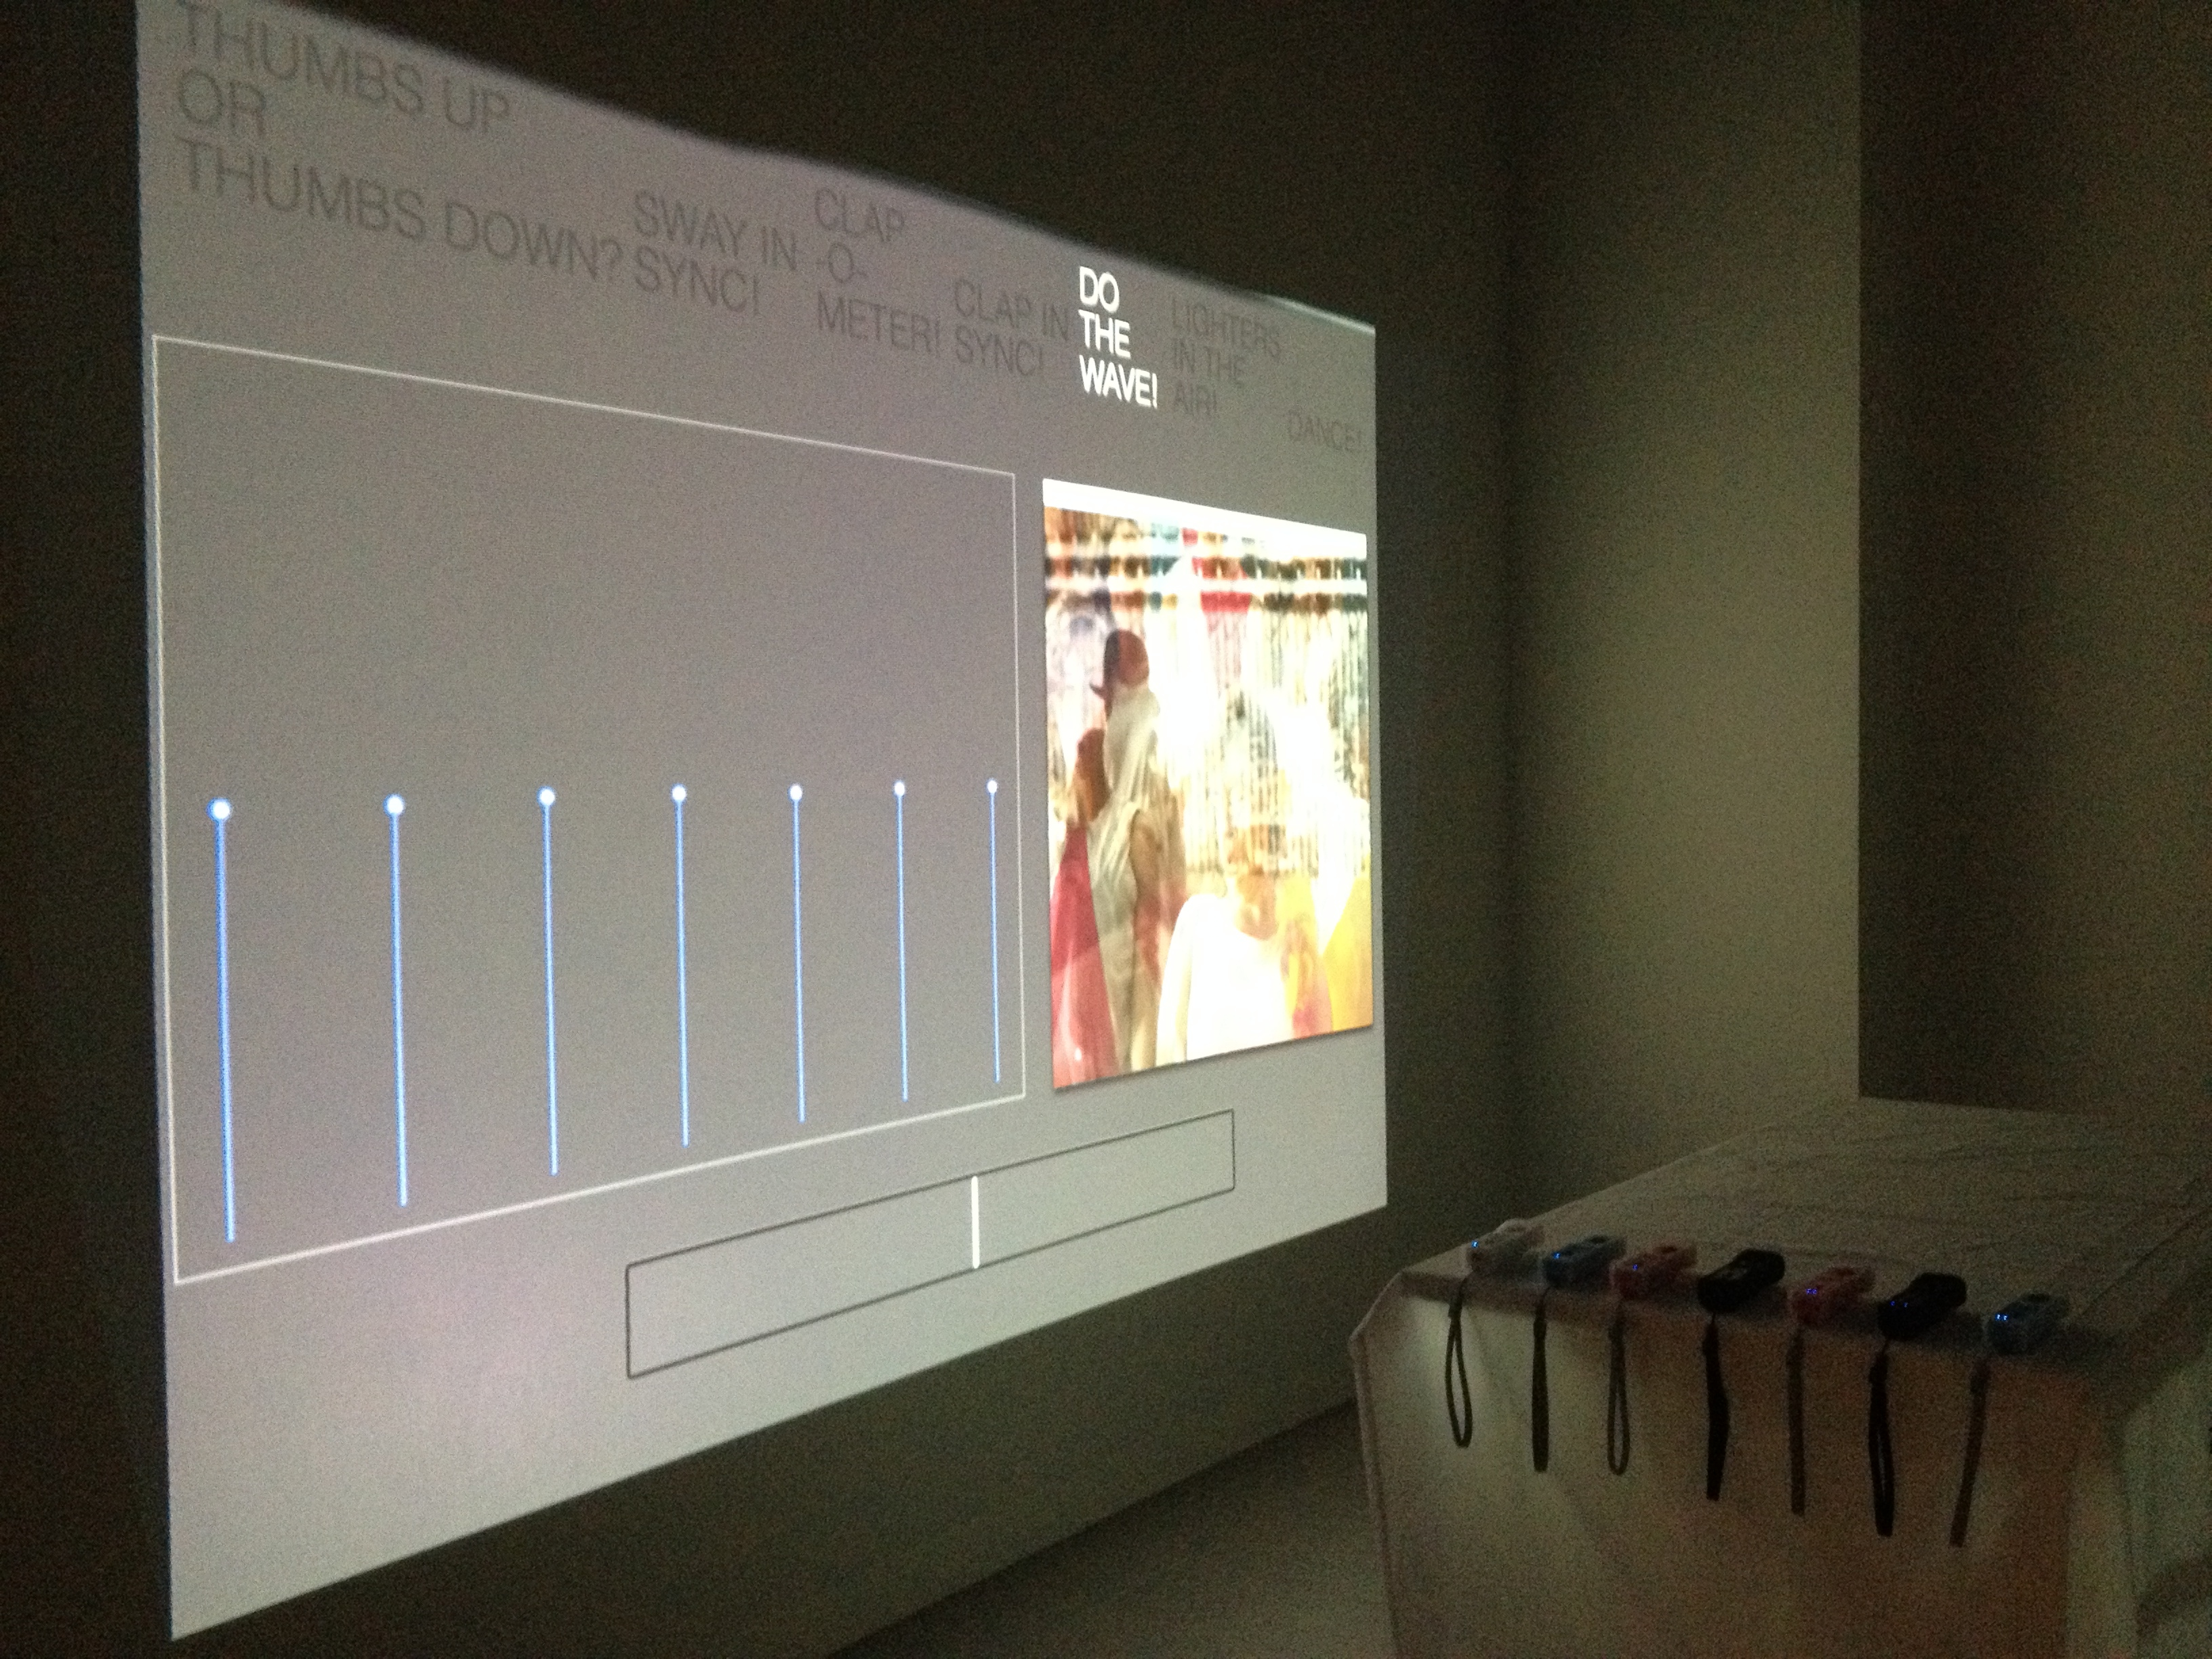
\includegraphics[height=0.3\textwidth]{eleo_live.jpg}
	\caption{The prototype on display at eLeo}

	\label{prototyping2.4}
\end{figure}


\section{Testing}
% Explain the details of how participants were recruited, how data was collected, recorded, and processed/analyzed, and the timeline over which this process unfolded

I watched users interacting with this prototype at the eLeo event. My prototype was set up in a room with a wall-sized projection. Here, my goal was to observe how users approached the technology and how multiple people performed the various inputs as a group...


\section{Analysis}
